% Copyright 2004 by Till Tantau <tantau@users.sourceforge.net>.
%
% In principle, this file can be redistributed and/or modified under
% the terms of the GNU Public License, version 2.
%
% However, this file is supposed to be a template to be modified
% for your own needs. For this reason, if you use this file as a
% template and not specifically distribute it as part of a another
% package/program, I grant the extra permission to freely copy and
% modify this file as you see fit and even to delete this copyright
% notice. 



\documentclass{beamer}
\newcommand{\card}[1]{\vert{#1}\vert}
\newcommand{\magn}[1]{\vert{#1}\vert}
\usepackage{relsize}
\usepackage{hyperref}
% There are many different themes available for Beamer. A comprehensive
% list with examples is given here:
% http://deic.uab.es/~iblanes/beamer_gallery/index_by_theme.html
% You can uncomment the themes below if you would like to use a different
% one:
%\usetheme{AnnArbor}
%\usetheme{Antibes}
%\usetheme{Bergen}
%\usetheme{Berkeley}
%\usetheme{Berlin}
%\usetheme{Boadilla}
%\usetheme{boxes}
%\usetheme{CambridgeUS}
%\usetheme{Copenhagen}
%\usetheme{Darmstadt}
%\usetheme{default}
%\usetheme{Frankfurt}
%\usetheme{Goettingen}
%\usetheme{Hannover}
%\usetheme{Ilmenau}
\usetheme{JuanLesPins}
%\usetheme{Luebeck}
%\usetheme{Madrid}
%\usetheme{Malmoe}
%\usetheme{Marburg}
%\usetheme{Montpellier}
%\usetheme{PaloAlto}
%\usetheme{Pittsburgh}
%\usetheme{Rochester}
%\usetheme{Singapore}
%\usetheme{Szeged}
%\usetheme{Warsaw}

\title{Void Reduction in Self-Healing Swarms}

% A subtitle is optional and this may be deleted
\subtitle{(Using proximity detection)}

\author{Neil~Eliot\inst{1}, David~Kendall\inst{1}, Alun~Moon\inst{1}, Michael~Brockway\inst{1}, Martyn~Amos\inst{1}}
% - Give the names in the same order as the appear in the paper.
% - Use the \inst{?} command only if the authors have different
%   affiliation.

%\renewcommand\appendixname{Appendix}

\institute[Northumbria University] % (optional, but mostly needed)
{
  \inst{1}
  Department of Computer and Information Sciences\\
  University of Northumbria
  % \and
  % \inst{2}
  % Department of Theoretical Philosophy\\
  % University of Elsewhere
}
% - Use the \inst command only if there are several affiliations.
% - Keep it simple, no one is interested in your street address.

\date{ALife, 2019}
% - Either use conference name or its abbreviation.
% - Not really informative to the audience, more for people (including
%   yourself) who are reading the slides online

\subject{Void Reduction in Self-Healing Swarms}
% This is only inserted into the PDF information catalog. Can be left
% out. 

% If you have a file called "university-logo-filename.xxx", where xxx
% is a graphic format that can be processed by latex or pdflatex,
% resp., then you can add a logo as follows:

% \pgfdeclareimage[height=0.5cm]{university-logo}{university-logo-filename}
% \logo{\pgfuseimage{university-logo}}

% Delete this, if you do not want the table of contents to pop up at
% the beginning of each subsection:
% \AtBeginSubsection[]
% {
%   \begin{frame}<beamer>{Outline}
%     \tableofcontents[currentsection,currentsubsection]
%   \end{frame}
% }

% Let's get started
\begin{document}

\begin{frame}
  \titlepage
\end{frame}

\begin{frame}{Introduction}
  \tableofcontents
  % You might wish to add the option [pausesections]
\end{frame}

% Section and subsections will appear in the presentation overview
% and table of contents.
\section{Set the Ground Rules!}

\subsection{Swarm Rules}

\begin{frame}{Swarm Rules}
  \begin{itemize}
  \item {
    Swarms consist of many agents (mobile robots or drones) that interact according to a simple set of rules.
  }
  \item {
    We consider swarms of agents that:
    \begin{itemize}
      \item Do not require any another form of communication. 
      \item Capable of detecting their neighbours (proximity detection). 
    \end{itemize}
  }
  \item {
    Swarms can be made fault tolerant (resilient to agent loss).
  }
  \end{itemize}
\end{frame}

\section{Communications and/or Sensing}
\subsection{Communications}
\begin{frame}{Why no communications?}
  
  \begin{columns}
    \column{0.5\textwidth}
      \begin{itemize}
        \item {
          Communication propagation protocol overhead.
          \begin{itemize}
            \item $n_1 \rightarrow n_3$
            \item $n_1 \rightarrow n_2$
            \item $n_3 \rightarrow n_2$ (decision!) 
          \end{itemize}
        }
        \item {   
          Message propagation takes time which limits swarm size.
        }
      \end{itemize}
    \column{0.5\textwidth}
      \begin{figure}
        \begin{center}
          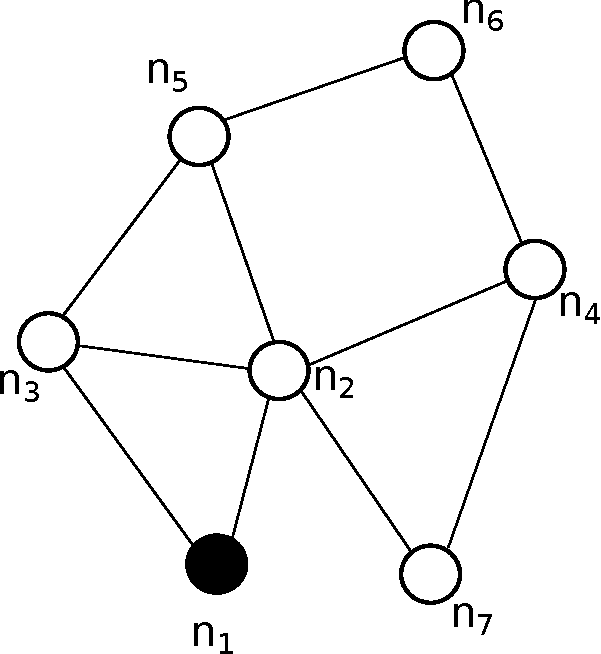
\includegraphics[width=2.5cm]{MessagePropogation1.pdf}
        \end{center}
      \end{figure}
      \begin{figure}
        \begin{center}
          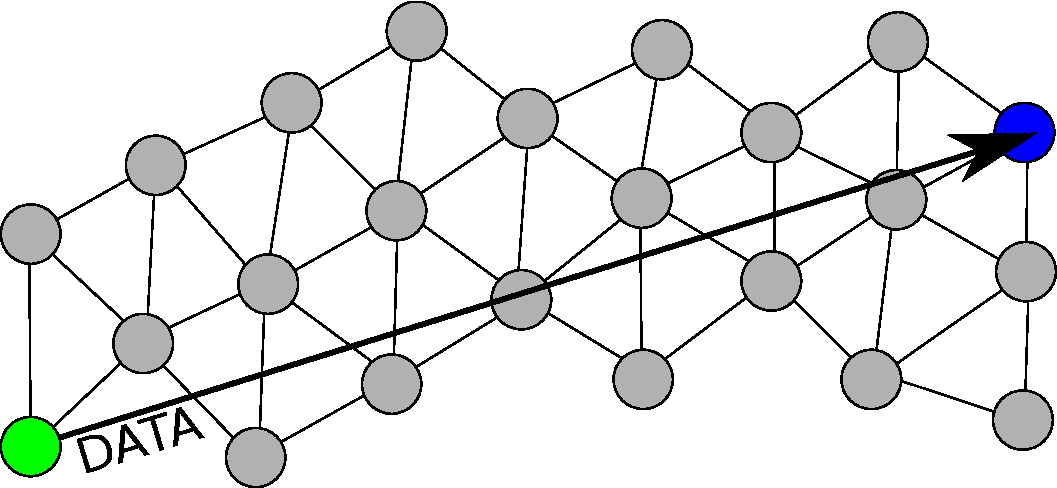
\includegraphics[width=4cm]{Comms1.pdf}
        \end{center}
        \caption{Swarm Communications}
      \end{figure}
    \end{columns}
\end{frame}

\subsection{Sensing}

\begin{frame}{Proximity Sensing}
  \begin{columns}
    \column{0.5\textwidth}
    \begin{itemize}
      \item {
        Proximity detection only, no other form of communication required.
      }
      \item {   
        Arbitrary sized swarms possible.
      }
      \item {   
        Agent attributes include various ranges (as shown in figure).
      }
    \end{itemize}
      \column{0.5\textwidth}
      \begin{figure}
        \begin{center}
        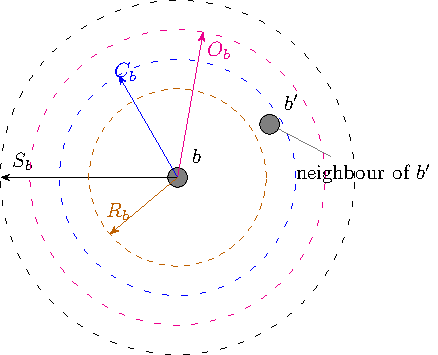
\includegraphics[width=5cm]{Proximity.pdf}
        \end{center}
        \caption{Ranges - $R_b$ - repulsion, $C_b$ - cohesion, $S_b$ - sensing, and $O_b$ - obstacles avoidance.}
      \end{figure}
  \end{columns} 
\end{frame}

\begin{frame}{Agent Movement}
  \begin{equation}\label{eq:BotPhysics1}
    v(b) = k_cv_c(b) + k_rv_r(b) + k_dv_d(b) + k_ov_o(b)
  \end{equation}
  \begin{itemize}
    \item $v_c(b)$ - cohesion to ensure agents remain part of the swarm.
    \item $v_r(b)$ - repulsion to ensure agents do not collide.
    \item $v_d(b)$ - destination vector for goal based swarms.
    \item $v_o(b)$ - obstacle avoidance vector.
    \item $k_c, k_r, k_d, k_o$ are weightings to allow modifications to the vector effects. 
  \end{itemize}
  
\end{frame}

\begin{frame}{The Swarm}
  \begin{figure}
    \begin{center}
      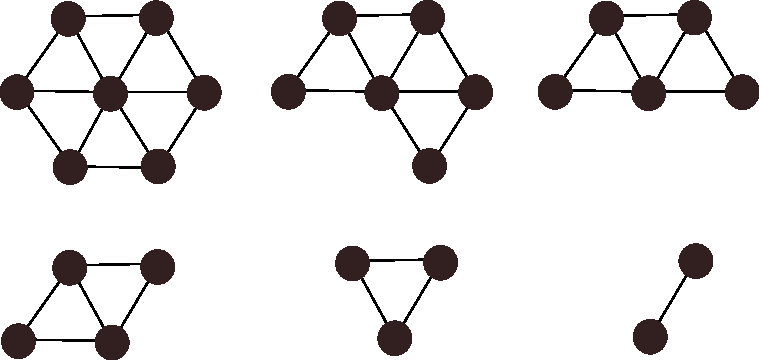
\includegraphics[width=4cm]{StableForms.pdf}
    \end{center}
    \caption{Stable Structures}
  \end{figure}
  \begin{figure}
    \begin{center}
      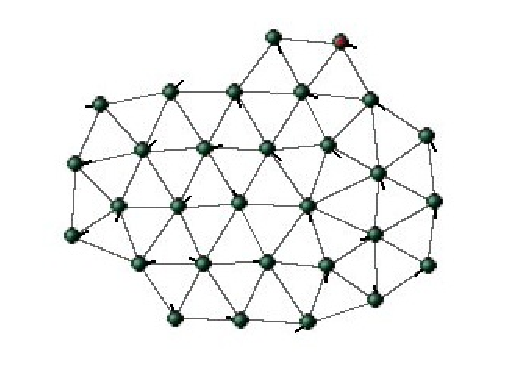
\includegraphics[width=4cm]{Stable.eps}
    \end{center}
    \caption{The Swarm - (Simulator)}
  \end{figure}
\end{frame}

\section{Void Reduction}

\subsection{Model}

\begin{frame}{Perimeter Detection}
  \begin{block}{NOTE}
    Perimeter detection is used as part of the \textit{void reduction} process. This will be discussed later. 
  \end{block}
  \begin{itemize}
    \item Perimeter detection allows for directional coordination with reduced resource usage.
      \begin{itemize}
        \item `Internal' agents don't need to use their GPS.
      \end{itemize}
    \item Reduces computational overhead in agents.
  \end{itemize}
\end{frame}

\begin{frame}{What is a Perimeter?}
  \begin{figure}
    \begin{center}
      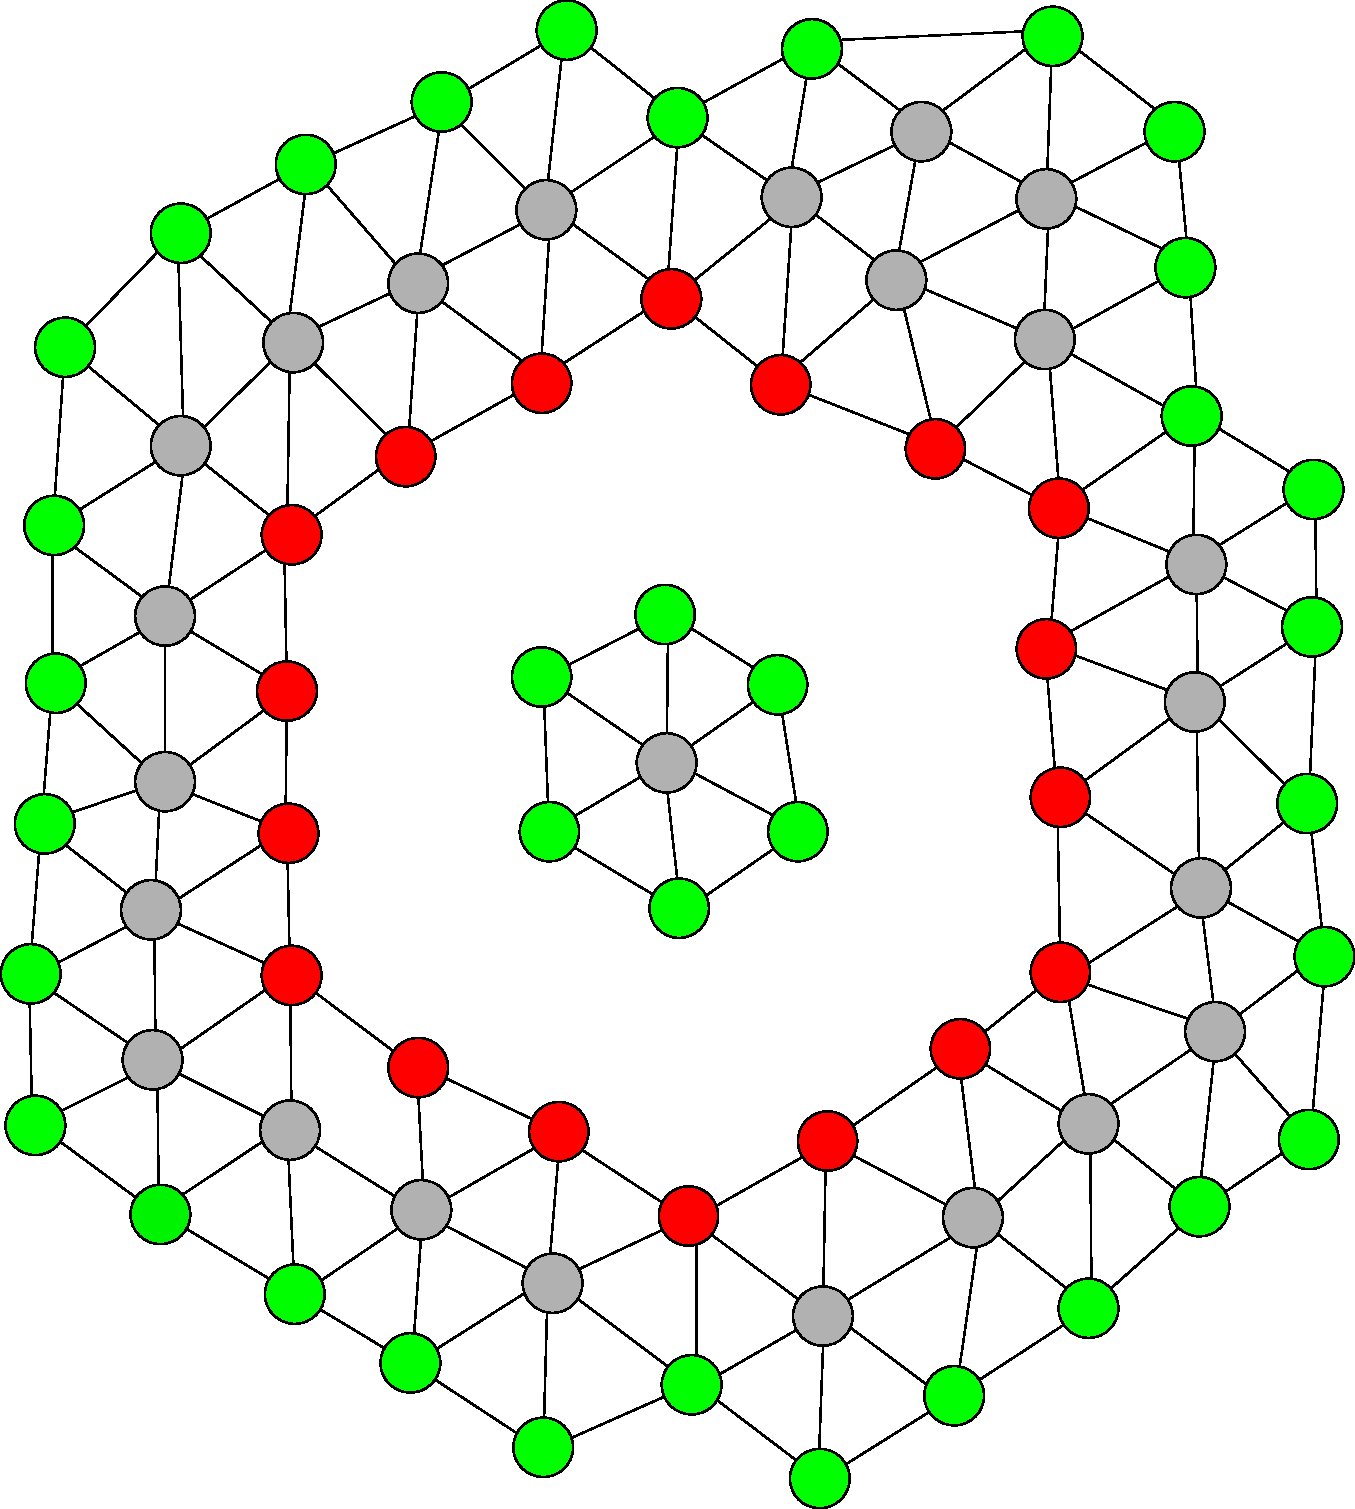
\includegraphics[width=5cm]{Perimeters.pdf}
    \end{center}
    \caption{Internal and external perimeters}
  \end{figure}
\end{frame}


\begin{frame}{Perimeter Detection (Concave)}
  \begin{figure}
    \begin{center}
      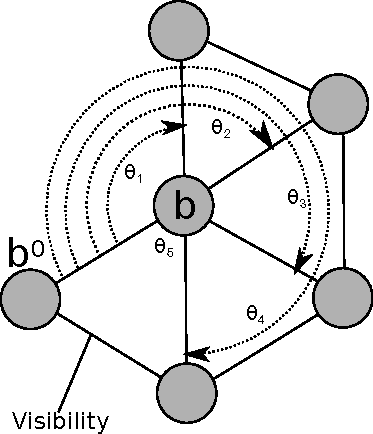
\includegraphics[width=5cm]{Perimeter1.pdf}
    \end{center}
    \caption{Concave gap (\textit{Void Reduction})}
  \end{figure}
\end{frame}

\begin{frame}{Perimeter Detection (Convex)}
  \begin{figure}
    \begin{center}
      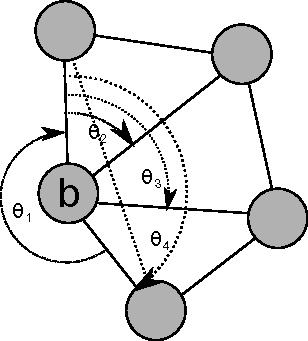
\includegraphics[width=5cm]{Perimeter2.pdf}
    \end{center}
    \caption{Convex gap}
  \end{figure}
\end{frame}

\begin{frame}{Void Reduction Movement}
  \begin{columns}
  \column{0.5\textwidth}
    \begin{figure}
      \begin{center}
        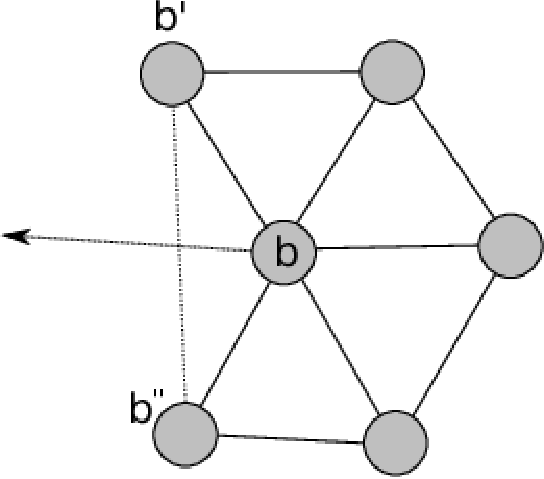
\includegraphics[width=5cm]{VoidConcave1.pdf}
      \end{center}
      \caption{Concave detection}
    \end{figure}
  \column{0.5\textwidth}
    As part of the perimeter detection a set ($G_b$) of agents is generated. This set is the first two agents identified as creating a `gap' in agent $b$'s neighbours. Equation~\ref{eq:ConcaveVoidPhysics3} calculates the centroid of the identified `gap'.
    \begin{center}
      \begin{equation}‎
      D_{pos}(b)=\frac{1}{2}\mathlarger{\sum_{b' \in G_b}}{b'}
      \label{eq:ConcaveVoidPhysics3}‎
      \end{equation}
    \end{center}
  \end{columns}
\end{frame}

\subsection{Local Effect}
\begin{frame}{Agent movement}
  \begin{columns}
    \column{0.5\textwidth}
      \begin{figure}
        \begin{center}
          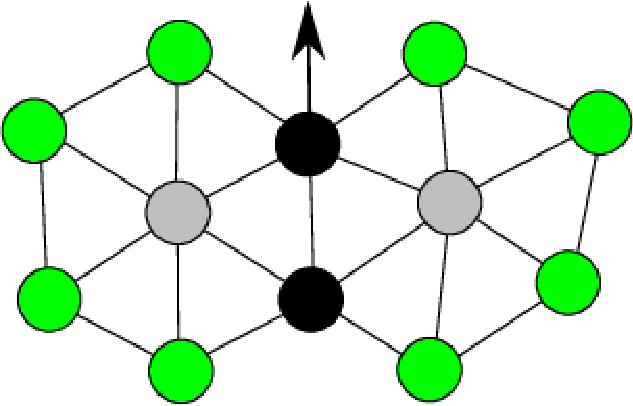
\includegraphics[width=5cm]{InterAgentEffect1.pdf}
        \end{center}
        \caption{Initial positions}
      \end{figure}
    \column{0.5\textwidth}
        \begin{figure}
          \begin{center}
            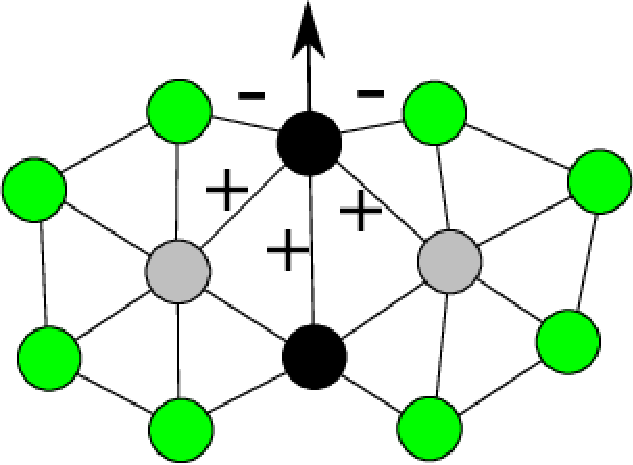
\includegraphics[width=5cm]{InterAgentEffect2.pdf}
          \end{center}
          \caption{Agent movement}
        \end{figure}
    \end{columns}
\end{frame}

\subsection{Global Effect}
\begin{frame}{Agent movement}
  \begin{columns}
    \column{0.5\textwidth}
      \begin{figure}
        \begin{center}
          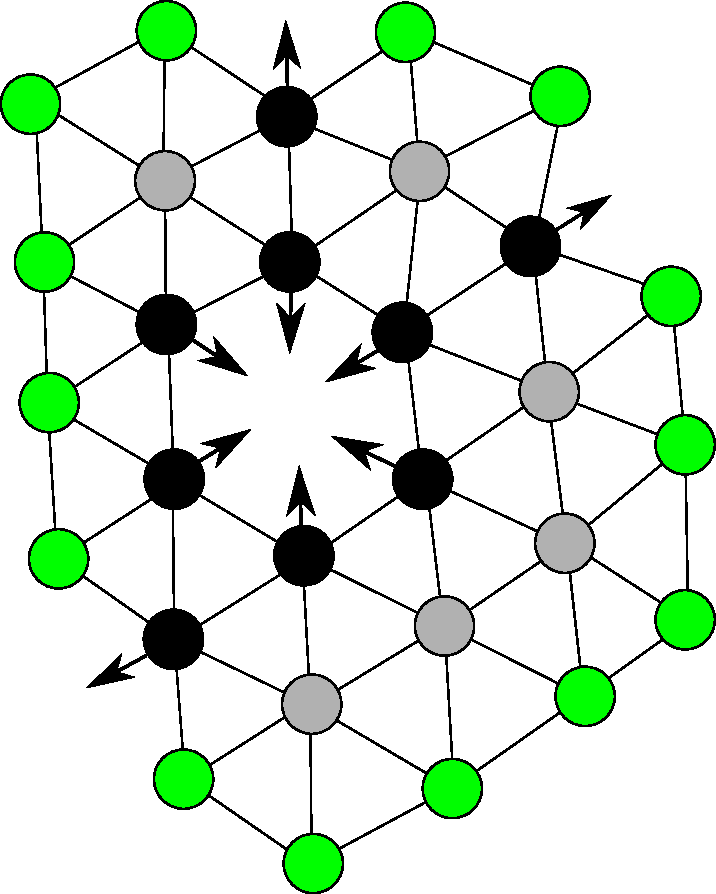
\includegraphics[width=5cm]{PerimeterBotsCircle3.pdf}
        \end{center}
        \caption{Initial positions}
      \end{figure}
    \column{0.5\textwidth}
        \begin{figure}
          \begin{center}
            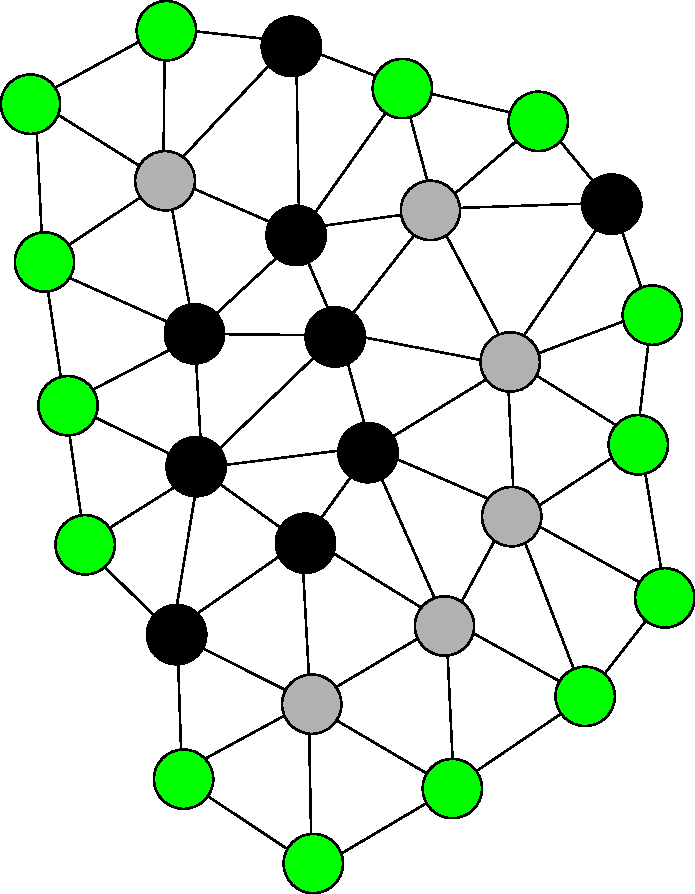
\includegraphics[width=5cm]{PerimeterBotsCircle4.pdf}
          \end{center}
          \caption{Agent movement}
        \end{figure}
    \end{columns}
\end{frame}  

\subsection{Simulated Results}
\begin{frame}{Scenario}
  \begin{center}
    \begin{figure}
      \begin{center}
        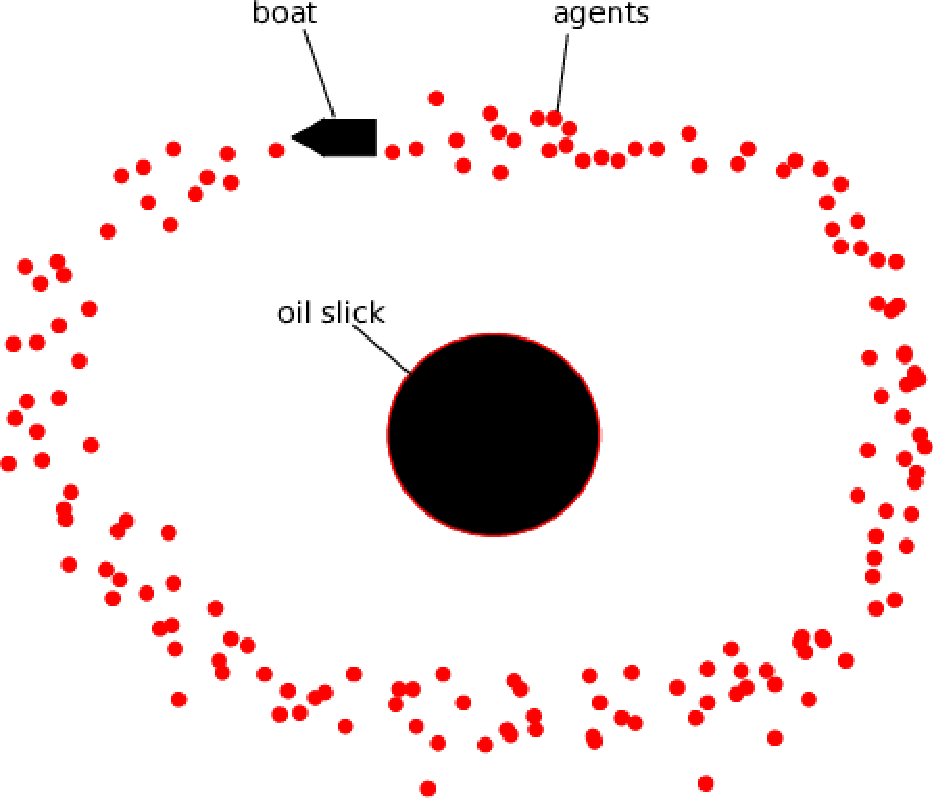
\includegraphics[width=7cm]{OilSlick.pdf}
      \end{center}
      \caption{Oil Slick Encapsulation}
    \end{figure}
  \end{center}
\end{frame}  

\begin{frame}{Video}
  \begin{center}
    \begin{figure}
      \begin{center}
        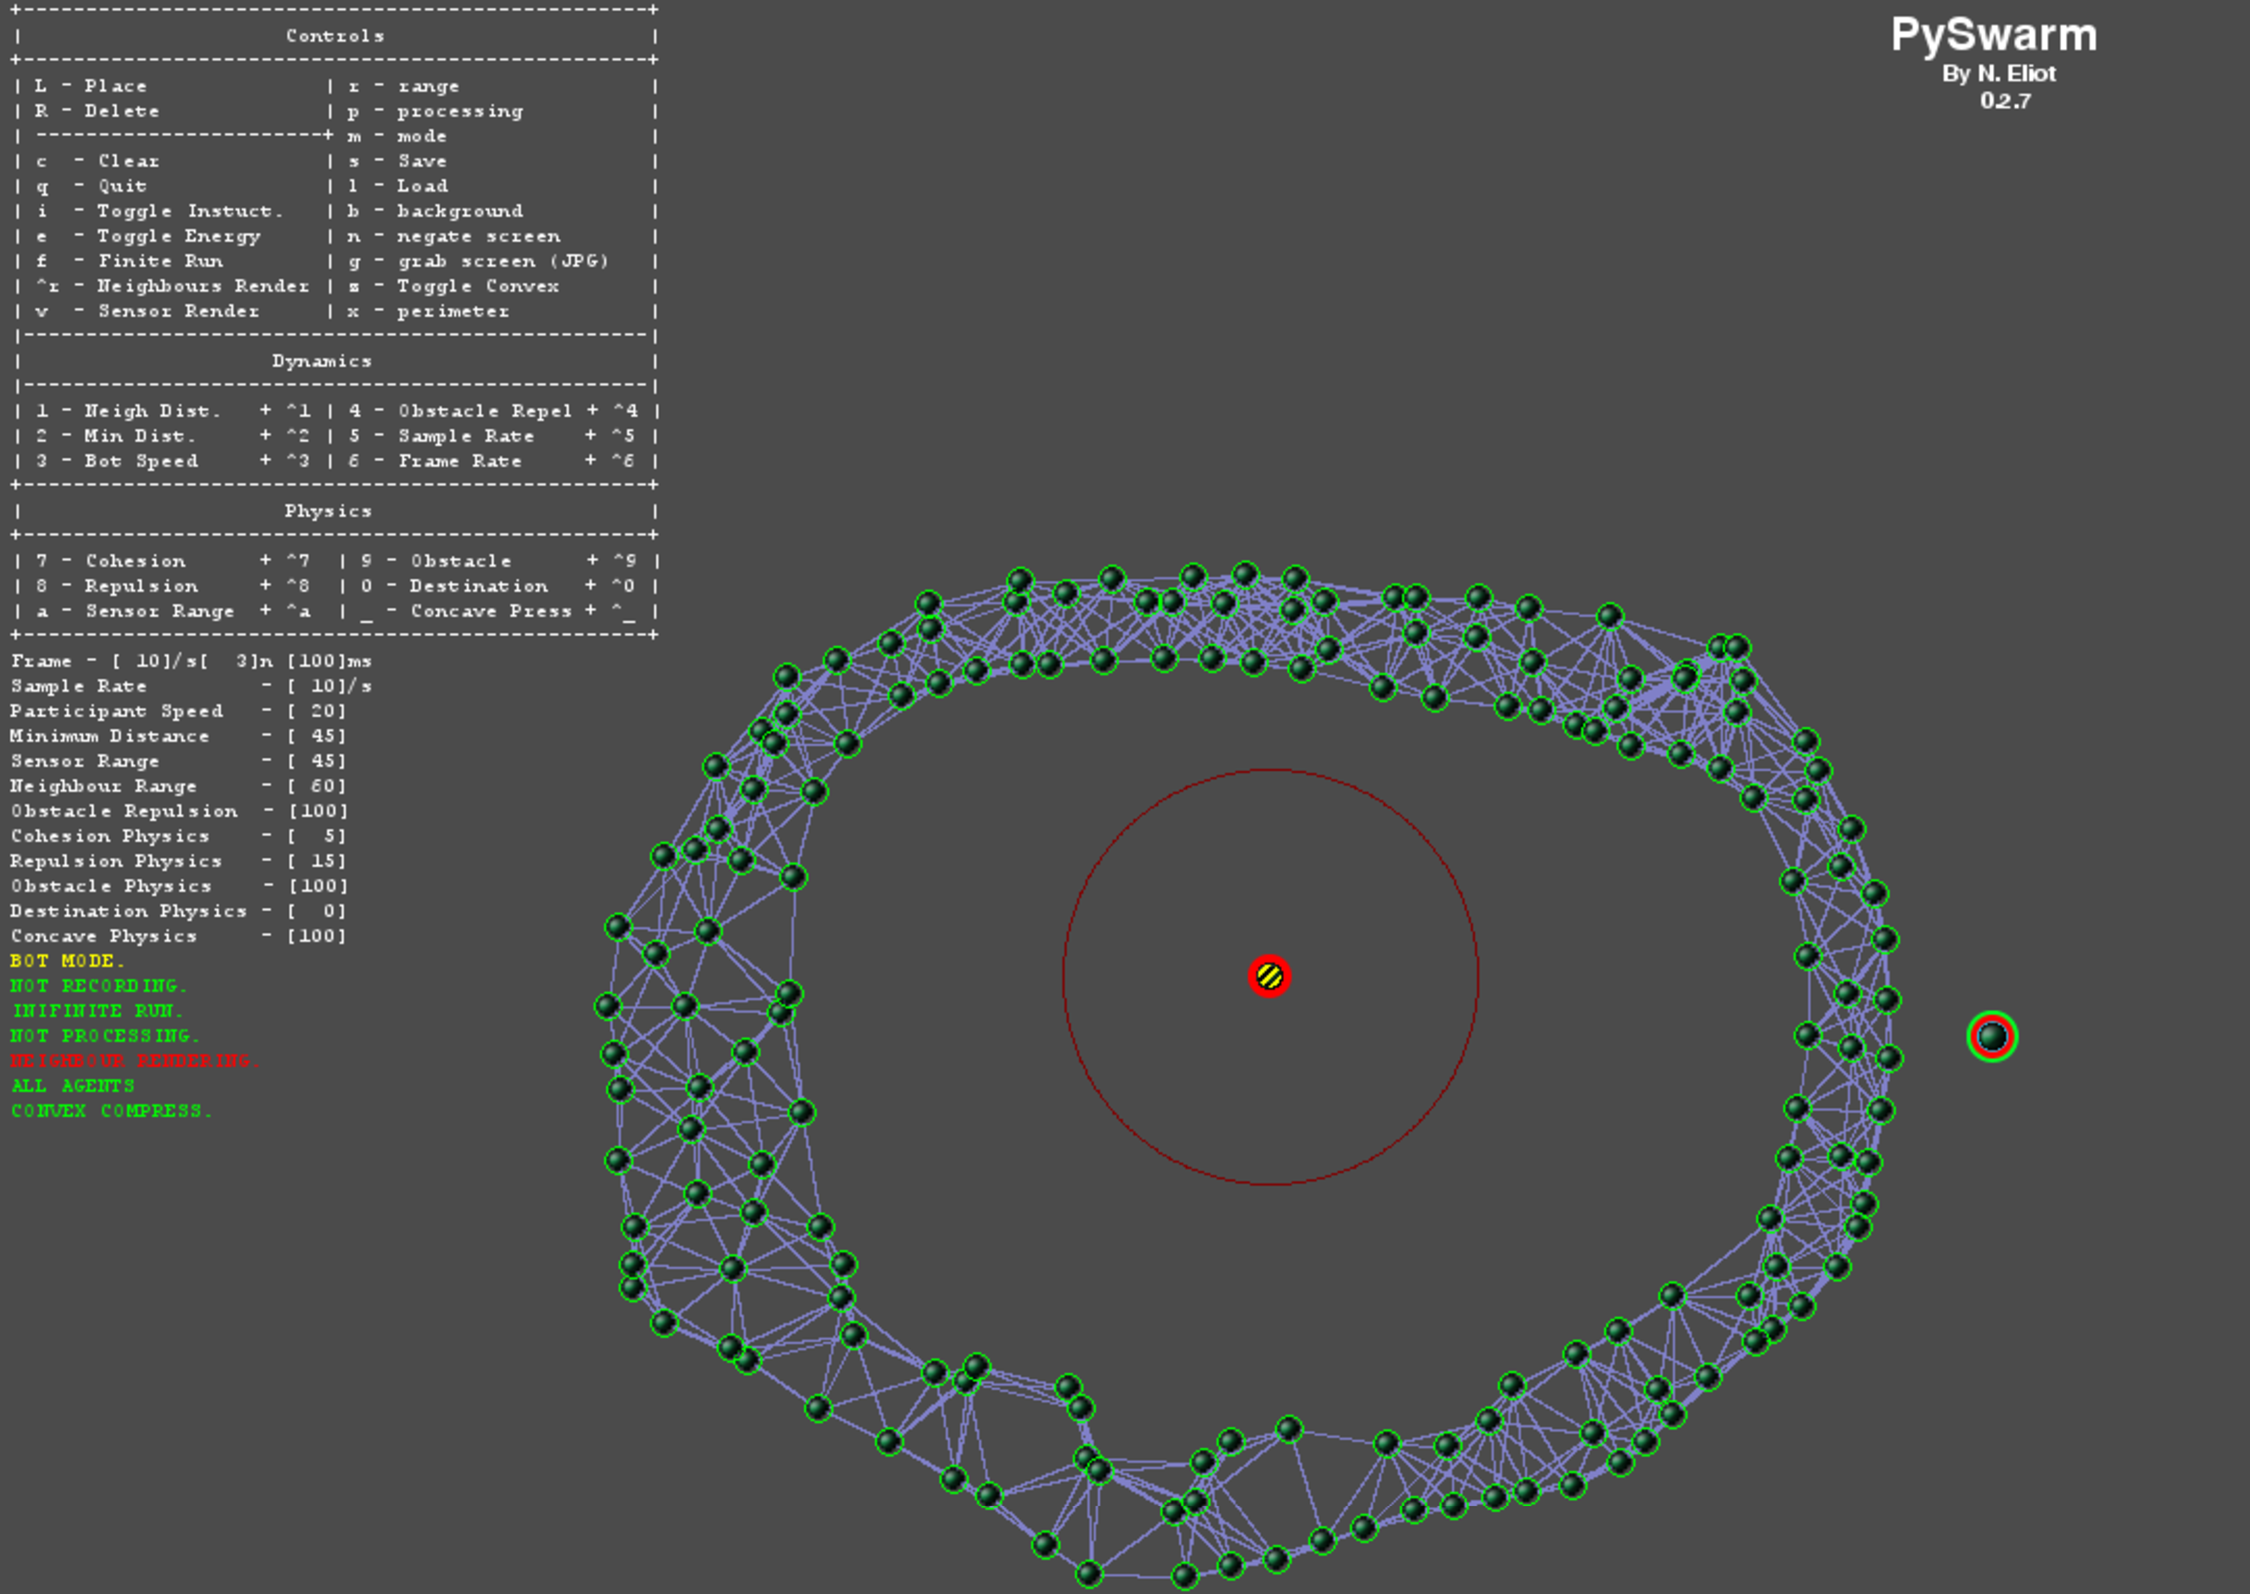
\includegraphics[width=7cm]{Simulator.pdf}
      \end{center}
      \caption{Simulator}
    \end{figure}
    \href{https://www.youtube.com/watch?v=iyMSpj10elk}{https://www.youtube.com/watch?v=iyMSpj10elk}
  \end{center}
\end{frame}  

% Placing a * after \section means it will not show in the
% outline or table of contents.  

\section*{Summary}

\begin{frame}{Summary}
  \begin{itemize}
  \item
    \alert{Void reduction} has a local effect creating a global emergent behaviour that improves the shape and structure of a swarm.
  \item
    \alert{Void reduction} removes anomalies on internal and external perimeters.
  \item
    \alert{Void reduction} can be applied to both static swarms and directional swarms.
  \end{itemize}
\end{frame}

\section*{Thank You}

\begin{frame}{Thank You}
  \begin{center}
  THANK YOU!\\
  QUESTIONS?
  \end{center}
\end{frame}

\section*{Appendix}

\begin{frame}{Agent Movement}
  \begin{equation}\label{eq:Repulsion1}
    v_r(b) = 
    \frac{1}{\card{\mathcal R_b}}
    \left(
      \mathlarger{\mathlarger{\sum_{b' \in \mathcal R_b}}}
      {\left( 1-\frac{\magn{b'}}{R_b} \right)}
      b'
    \right)
    \end{equation}
    \begin{equation}\label{eq:FlyToCentre1}
      v_c(b) =
      \frac{-1}{\card{\mathcal C_b}}\left({\mathlarger{\sum_{b' \in
      \mathcal C_b}}{b'}}\right)
    \end{equation}
\end{frame}

\begin{frame}{Agent Movement}
    \begin{equation}\label{eq:Direction}
      v_d(b) = d
    \end{equation}
    \begin{eqnarray}\label{eq:Obstacle2}
      v_o(b) & = & O_b \hat q_o \\
      \mathrm{where~}  q_o & = & \sum_{o\in \mathcal O_b } \hat o
      \nonumber \\
      v_o(b) & = & O_b \left(\sum_{o\in \mathcal O_b }\hat o\right)^{\!\!\wedge} \nonumber
    \end{eqnarray}
\end{frame}

\end{document}


